\section{Query Approximation}
\label{sec-query}



\begin{figure}[tb!]
  \vspace{-1ex}
  \begin{center}
  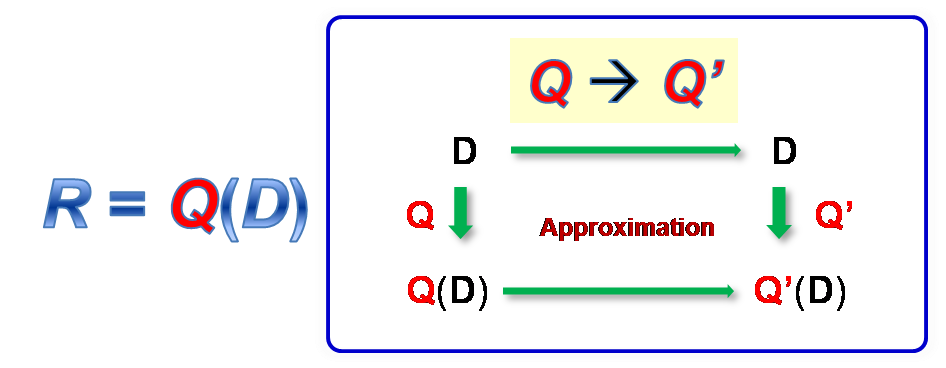
\includegraphics[scale=0.45]{./queryApprox.png}
  \end{center}
  \vspace{-3ex}
  \caption{Query approximation}\label{fig-tech-queryappro}
  \vspace{-2ex}
\end{figure}


Query approximation deals with complex queries involved with big data analytic tasks. Given a class $Q$ of data analytic queries with higher computational complexity,  query approximation is to transform into another class $Q'$ of queries with lower computational complexity and satisfiable approximate answers, as depicted in Fig.~\ref{fig-tech-queryappro} in which $Q$, $Q'$ and $D$ denote the original query, approximate query and data, respectively. Query approximation needs to reach a balance between the query efficiency and answer accuracy when approximating $Q$ with $Q'$.

The rationale behind query approximation has inexact or approximate answers are acceptable for many big data analytic tasks.
On one hand, when the volume of data is extremely large, it may be impossible or not necessary to compute the exact queries.
Observe that nobody would try each and every store to find a pair of shoes with the best cost-performance ratio.
That is, inexact (approximate) solutions are good candidates in this case.
%
On the other hand, when taking noises (common for big data) into account, it may not always a good idea to compute exact answers
for those data analytic tasks whose answers are rare or hard to identify, such as the detection of homegrown violent extremists (HVEs) who seek to commit acts of terrorism in the United States and abroad~\cite{HungJ16}, as exact solutions may have a high chance to miss possible candidates.

We next explain query approximation computation in more detail with three different data analytic tasks.



\stitle{(1) Strong simulation~\cite{tods-MaCFHW14}}. Given a pattern graph $Q$ and a data graph $G$,
{\em Graph pattern matching} is to find all subgraphs of $G$ that match $Q$, and is being increasingly used in various applications, \eg software, biology, social networks and intelligence analysis.


Here {\em matching} is typically defined in terms of
{\em subgraph isomorphism} \cite{Galla06}:
a subgraph $G_s$ of $G$ {\em matches} $Q$ if
there exists a {\em bijective function} $f$
from the nodes of $Q$ to the nodes in $G_s$ such that (a)  for each
pattern node $u$ in $Q$, $u$ and $f(u)$
have the same label,
and (b) there exists an edge $(u, u')$ in $Q$ if and only
if there exists an edge $(f(u), f(u'))$ in $G_s$.


The goodness of subgraph isomorphism is that all matched subgraphs  are exactly the same as the pattern graph, \ie completely preserving the  topology structure between the pattern graph and data graph. However, subgraph isomorphism is \NP-complete, and may return exponential many matched subgraphs.
Further, subgraph isomorphism is too restrictive to find sensible matches in certain scenarios, as observed in~\cite{FanLMTWW10}. Even worse, online data in many cases only represents a partial world (\eg terrorist collaboration networks and homosexual networks often involve with a large amount of off-line data).
Exact computations on such online data, whose accompanying off-line data is extremely hard to gather, typically decreases the chance of identifying candidate answers.
These hinder the usability of graph pattern matching in emerging applications.


To lower the high complexity of subgraph isomorphism, substitutes for subgraph isomorphism~\cite{FanLMTWW10,FanLMTW11} that allow graph pattern matching to be conducted in cubic-time have been proposed by extending graph simulation~\cite{infsimu95}. However, they fall short of capturing the topology of data graphs, i.e., graphs may have a structure drastically different from pattern graphs they match, and the matches found are often too large to analyze.

To rectify these problems, strong simulation, an ``approximate'' substitute for subgraph isomorphism, was  proposed for graph pattern matching, such that strong simulation (a) theoretically preserves the key topology of pattern graphs and finds a bounded number of matches, (b) retains the same complexity as earlier extensions of graph simulation~\cite{FanLMTWW10,FanLMTW11}, by providing a cubic-time algorithm for computing strong simulation, and (c) has the locality property that allows us to develop an effective distributed algorithm to conduct graph pattern matching on distributed graphs~\cite{tods-MaCFHW14}.

Strong simulation is experimentally verified that it is able to identify sensible matches that are not found by subgraph isomorphism, and it finds high
quality matches that retain graph topology. Indeed, 70\%-80\% of matches found by subgraph
isomorphism are retrieved by strong simulation, without paying the price of intractable complexity (100+ times faster) and large number (or
size) of matches.



\stitle{(3) One-pass Trajectory Compression~\cite{LinMZWH17}}. Nowadays, various sensors are collecting, storing and transmitting
tremendous trajectory data, and it is known that raw trajectory data seriously wastes the storage, network
band and computing resource.  Trajectory Compression techniques are an effective approach to attacking this issue by
compressing data points in a trajectory to a set of continuous
line segments, and are commonly used in practice.

 Though lossless compression methods have no information loss, their compression ratios are poor and queries on the compressed data are time consuming because data reconstructions from the compressed data are typically needed before the queries \cite{Nibali:Trajic} .
Hence, A large number of lossy trajectory compression techniques, most notably the piece-wise line simplification, have been developed.
These techniques focus on good compression ratios with bounded errors, and are the mainstream techniques for trajectory compression.
The idea of piece-wise line simplification (\lsa) comes from computational geometry, whose target is to approximate a given finer piece-wise linear curve by another coarser piece-wise linear curve ({normally} a sub set of the former), such that the maximum distance of the former from the later is bounded by a user specified constant. It is widely used due to its distinct advantages: (a) simple and easy to implement, (b) no need of extra knowledge and suitable for freely  moving  objects, and (c) bounded errors with good compression ratios.


The \lsa algorithms solving the \emph{min-$\#$} problem fall into two categories: {\em optimal} and {\em sub-optimal}.
The \textit{optimal} methods\cite{Imai:Optimal} are to find the minimal number of points or segments to represent the original polygonal lines \wrt an error bound $\epsilon$. The optimal \lsa algorithms have relative high time/space complexities which make them impractical for large trajectory data.
Hence, \textit{sub-optimal} \lsa algorithms have been developed and/or introduced for trajectory compression, including batch algorithms (\eg \cite{Douglas:Peucker}), online algorithms (\eg~\cite{Liu:BQS}) and one-pass algorithms (\eg~\cite{LinMZWH17}).


 We first develop a one-pass error bounded trajectory simplification algorithm that runs in $O(n)$ time and $O(1)$ space. \operb is based on a novel local distance checking method, and equipped with five optimization techniques to further improve its compression ratio. Essentially, fitting function: property...

\stab (2) We then propose an aggressive one-pass error bounded trajectory simplification algorithm (\operab) that remains in $O(n)$ time and $O(1)$ space.
\operba allows interpolating new data points into a trajectory under certain conditions and with practical considerations. The rational lies in that moving objects  have sudden track changes while data points may  not be sampled due to various reasons.

 finally conduct an extensive experimental study, by comparing our algorithms \operaa and \operab with \fbqsa (\emph{the fastest} existing \lsa algorithm) and \dpa (the {\em best} existing \lsa algorithm in terms of {\em compression ratio}). We find that \operaa and \operab are on average $(4.1, 4.1, 5.4, 5.2)$ times faster than \fbqsa on , respectively.
For compression ratios, \operaa is comparable with \dpa, and \operab is better than \dpa that is on average ($84.2\%, 86.4\%, 97.1\%, 94.7\%$) of \dpa , respectively.


\stitle{(2) Dense Temporal Subgraph Computation~\cite{MaHWLH17}}. Dense subgraph discovery and analysis have been widely studied in static networks, such as  finding maximal cliques, k-core analysis and  the Prize Collecting Steiner Tree problem. It is worth pointing out that dense subgraphs are a very general concept, and their concrete semantics highly depend on the studied problems and applications. How to properly transfer or define their semantics over to temporal networks is still in the early stage, not to mention effective and efficient analytic algorithms.

We investigate a special class of temporal networks (see a recent survey \cite{tn-survey}) such that their nodes and edges are kept fixed, but their edge weights constantly and regularly vary with timestamps. Essentially, a temporal network with $T$ timestamps can be viewed as $T$ snapshots of a static network such that the network nodes and edges are kept the same among these $T$ snapshots, while the edge weights vary with network snapthots.
%
Road traffic networks typically fall into this category, and  road traffic analyses are of particular importance for large cities, such as Beijing, New York, London and Paris, that are facing with heavy traffic congestions, one of the great challenges of urban computing.

We also focus on a certain form of dense temporal subgraphs, which was initially studied in \cite{BogdanovMS11}.
Formally speaking, a temporal subgraph corresponds to a connected subgraph measured by the sum of all its edge weights in a time interval, \ie  a continuous sequence of timestamps. Intuitively, a dense subgraph that we consider  corresponds to a  collection of connected highly slow or jam roads (\ie  a jam area) in road networks, lasting for a continuous sequence of snapshots.


However, the problem of  finding dense subgraphs in temporal networks is non-trivial, and it is already \NP-complete even for a temporal network with a single snapshot and with $+1$ or $-1$ edge weights only, as observed in \cite{BogdanovMS11}. Even worse, it remains hard to approximate for temporal networks  with single snapshots. Moreover, given a temporal network with $T$ timestamps, there are a total number of $T*(T+1)/2$ time intervals to consider, which further aggravates the difficulty. Finally, the state of the art solution {\sc meden} \cite{BogdanovMS11} adopts a filter-and-verification framework that {\em even if a large portion of time intervals are filtered, there often remain a large number of time intervals to verify}. Hence, {\sc meden} is not scalable when temporal networks have a large number of nodes/edges or a large number $T$ of timestamps.


 a highly efficient and effective data-driven approach, instead of filter-and-verification, which employs hidden data statistics to find dense temporal subgraphs in large temporal networks.  data-driven approach to identifying $k$ time intervals from a total of $T*(T+1)/2$ ones, striking a balance between quality and efficiency, in which $T$ is the number of snapshots and $k$ is a small constant, \eg 10. This is achieved by exploring the characteristics of time intervals involved with dense subgraphs based on a novel {\em evolving convergence phenomenon}.



Using both real-life and synthetic data, we conduct an extensive experimental study.
(a) We find that the dense subgraphs found by our method {\sc FIDES} have the best quality, \ie about 100.20\% and 100.15\% on average of those found by the state of the art solution {\sc meden}~\cite{BogdanovMS11}, respectively.
(b) Our method {\sc FIDES} is  on average 2,980 and 1,486 times  faster than {\sc meden}, respectively.
(c) Finally, {\sc meden} already ran out of memory for temporal graphs with 150,000 nodes and 2,000 snapshots only.


Temporal network -> dynamic road network -> dense temporal subgraph (definition) -> time interval (FAV)- not big data friendly

Temporal network analysis
has recently attracted more and more attentions
